\suppsection{S22. Secondary figures}
The following figures report secondary approximate-decoder, scalarized-cost, and effective-reliability diagnostics. Their original plotted data are unchanged. Their baselines and resource conventions differ from the matched pairwise theorem.
\begin{figure}[p]\centering
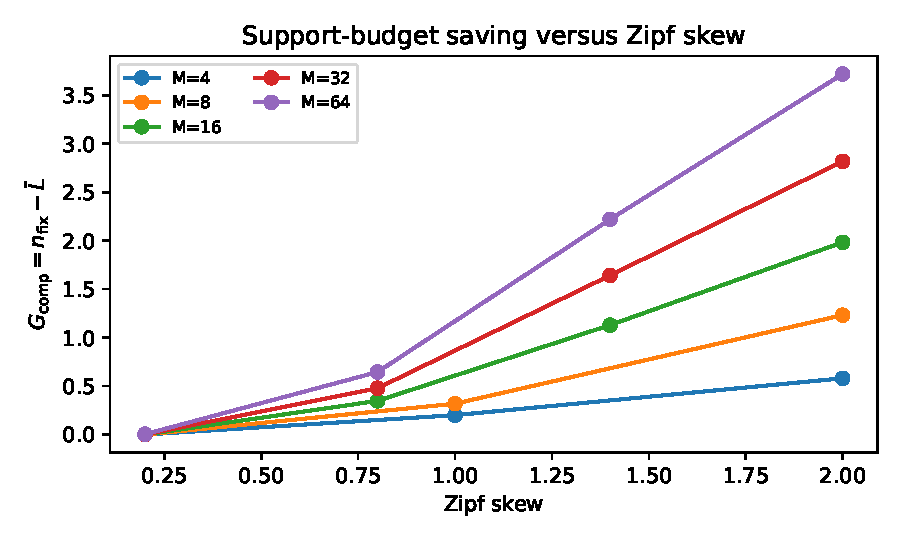
\includegraphics[width=0.86\linewidth,height=0.25\textheight,keepaspectratio]{figures/source_support_saving_vs_zipf.pdf}
\caption{Source-dependent average support-index allocation. This diagnostic reports a classical length-derived coordinate.}\label{fig:secondary-source_support_saving_vs_zipf}
\end{figure}
\begin{figure}[p]\centering
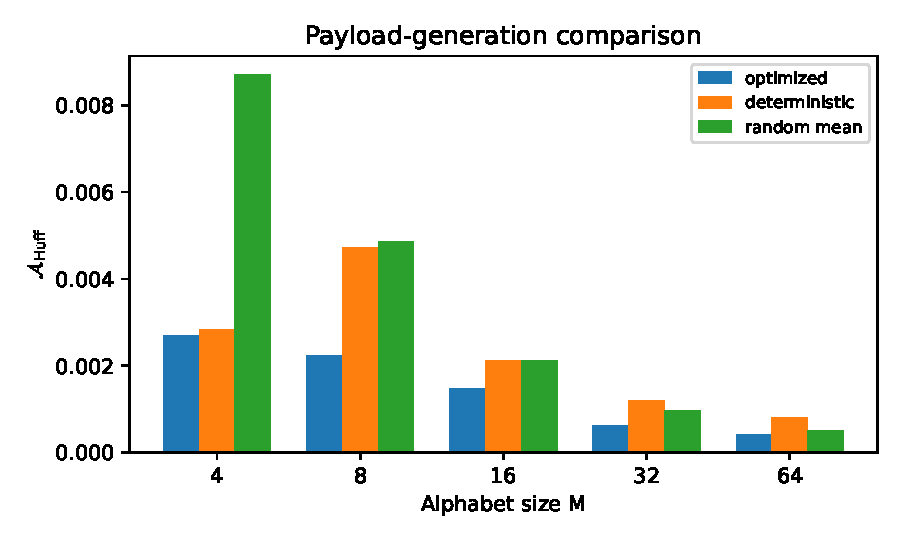
\includegraphics[width=0.86\linewidth,height=0.25\textheight,keepaspectratio]{figures/payload_generation_comparison.pdf}
\caption{Secondary payload-generation comparison with the original deterministic, random-phase, and local-search modes.}\label{fig:secondary-payload_generation_comparison}
\end{figure}
\begin{figure}[p]\centering
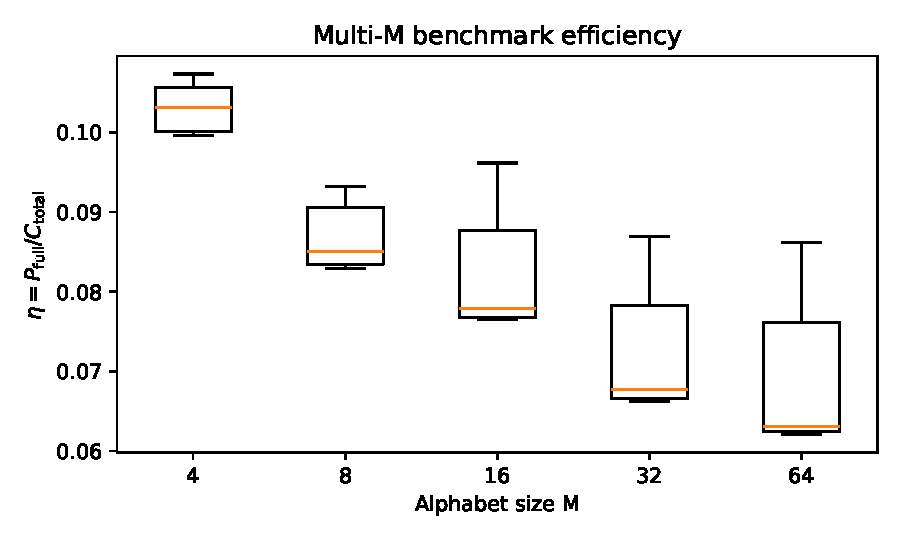
\includegraphics[width=0.86\linewidth,height=0.25\textheight,keepaspectratio]{figures/multiM_benchmark_efficiency.pdf}
\caption{Scalable PGM efficiency benchmark under the declared scalarized cost convention.}\label{fig:secondary-multiM_benchmark_efficiency}
\end{figure}
\begin{figure}[p]\centering
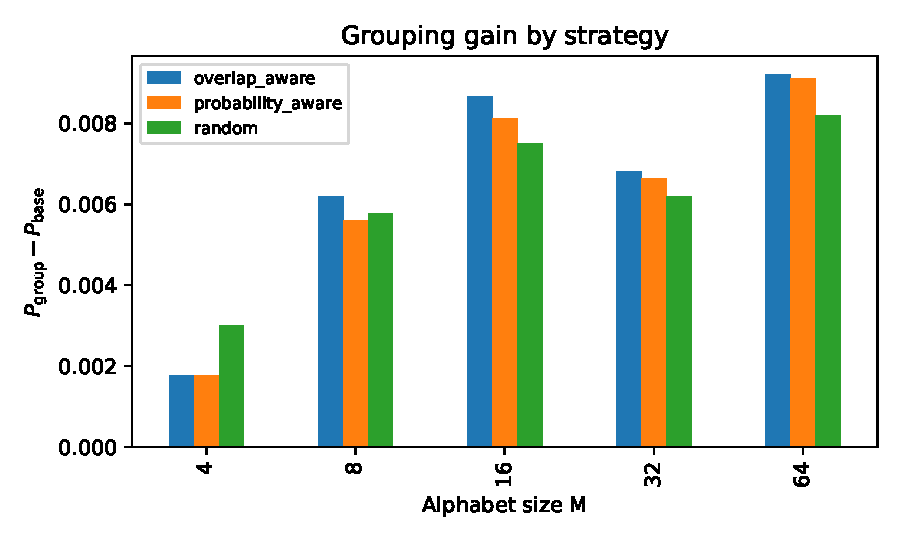
\includegraphics[width=0.86\linewidth,height=0.25\textheight,keepaspectratio]{figures/grouping_gain_by_strategy.pdf}
\caption{Secondary grouping comparison. Overlap-aware grouping is a geometry-dependent heuristic, outside the registered main comparison.}\label{fig:secondary-grouping_gain_by_strategy}
\end{figure}
\begin{figure}[p]\centering
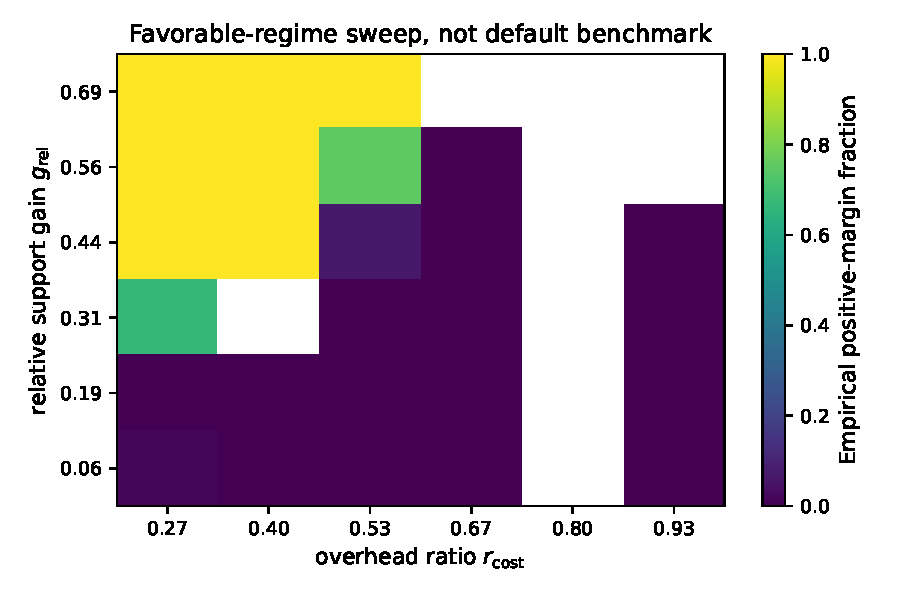
\includegraphics[width=0.86\linewidth,height=0.25\textheight,keepaspectratio]{figures/favorable_sweep_heatmap.pdf}
\caption{Finite sampled favorable-regime PGM diagnostic; the color scale is a convention-dependent scalar margin.}\label{fig:secondary-favorable_sweep_heatmap}
\end{figure}
\begin{figure}[p]\centering
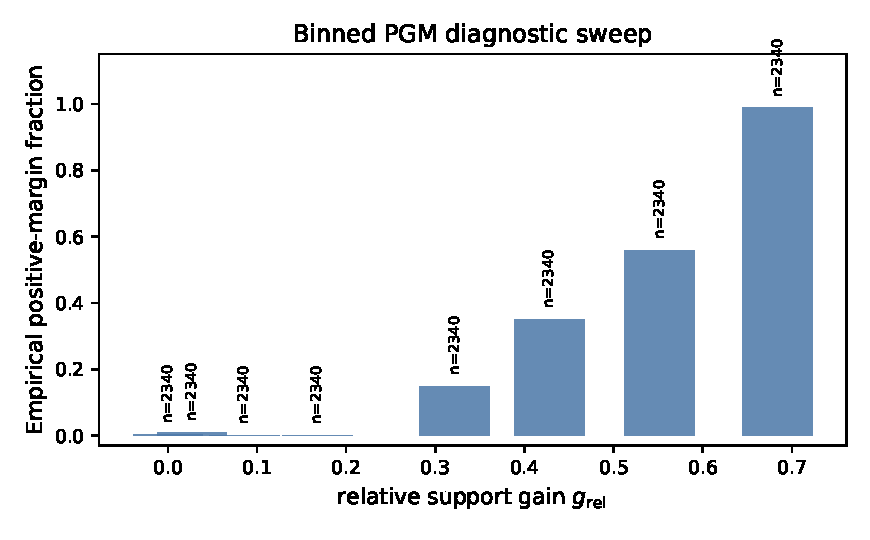
\includegraphics[width=0.86\linewidth,height=0.25\textheight,keepaspectratio]{figures/favorable_positive_fraction_vs_grel.pdf}
\caption{Finite sampled favorable-regime diagnostic versus relative support-index saving. Fractions describe sampled design rows.}\label{fig:secondary-favorable_positive_fraction_vs_grel}
\end{figure}
\begin{figure}[p]\centering
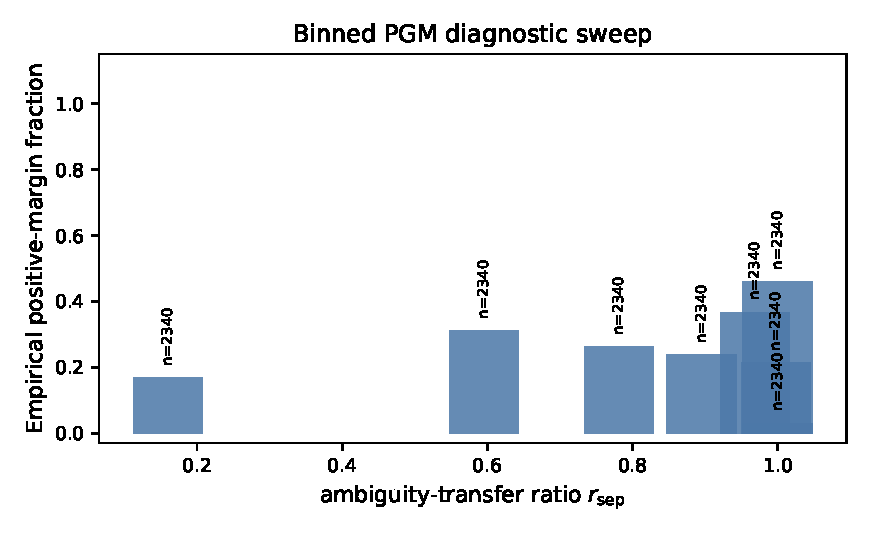
\includegraphics[width=0.86\linewidth,height=0.25\textheight,keepaspectratio]{figures/favorable_positive_fraction_vs_rsep.pdf}
\caption{Finite sampled favorable-regime diagnostic versus removed overlap ambiguity.}\label{fig:secondary-favorable_positive_fraction_vs_rsep}
\end{figure}
\begin{figure}[p]\centering
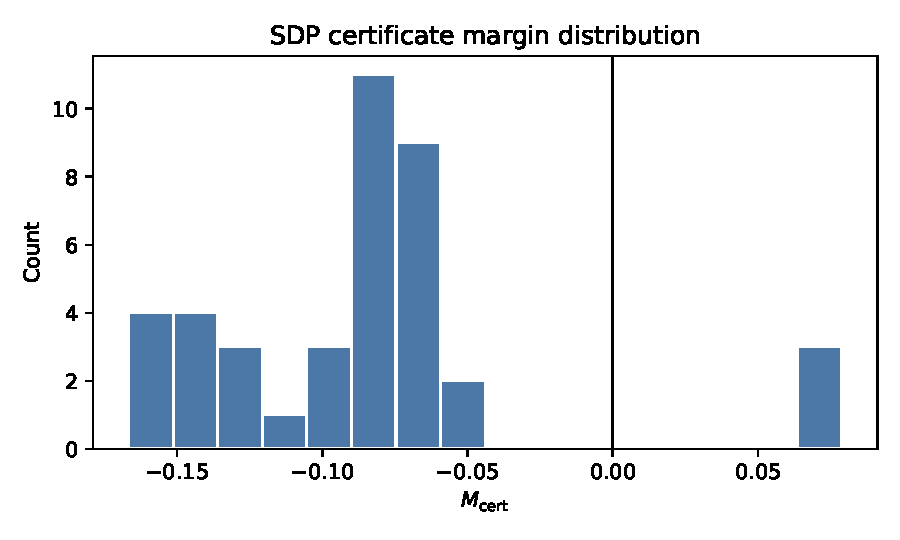
\includegraphics[width=0.86\linewidth,height=0.25\textheight,keepaspectratio]{figures/M_cert_distribution.pdf}
\caption{Secondary small-instance scalarized certificate margins. The fixed reference and accounting differ from the side-information-matched main comparison.}\label{fig:secondary-M_cert_distribution}
\end{figure}
\begin{figure}[p]\centering
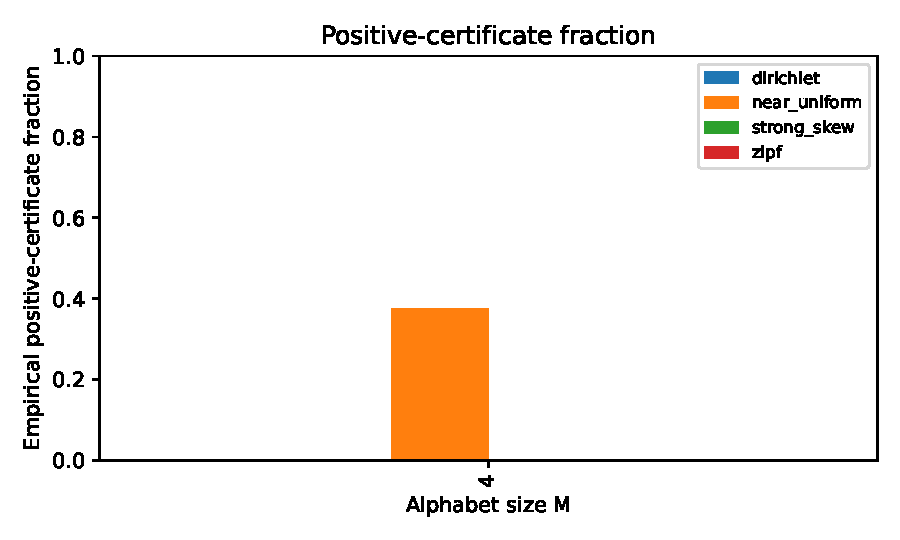
\includegraphics[width=0.86\linewidth,height=0.25\textheight,keepaspectratio]{figures/positive_certificate_ratio.pdf}
\caption{Secondary scalarized certificate fraction for the original finite sample; PGM rows are diagnostics.}\label{fig:secondary-positive_certificate_ratio}
\end{figure}
\begin{figure}[p]\centering
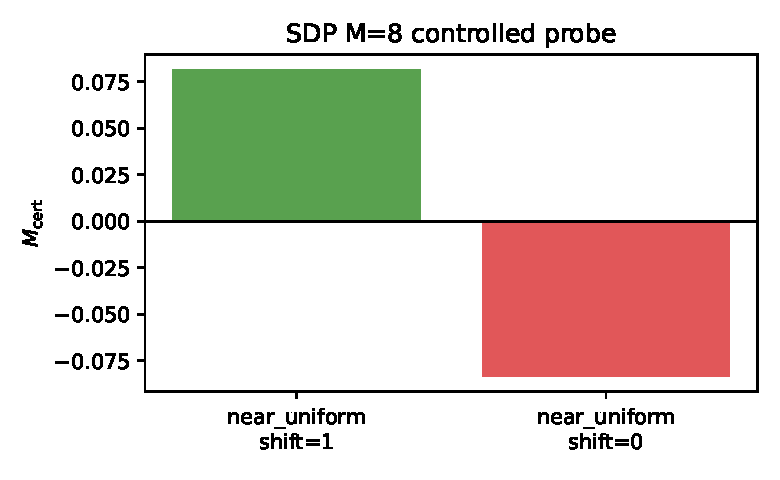
\includegraphics[width=0.86\linewidth,height=0.25\textheight,keepaspectratio]{figures/exact_sdp_m8_probe.pdf}
\caption{Two controlled secondary M=8 scalarized SDP certificate probes, distinct from the registered matched family.}\label{fig:secondary-exact_sdp_m8_probe}
\end{figure}
\begin{figure}[p]\centering
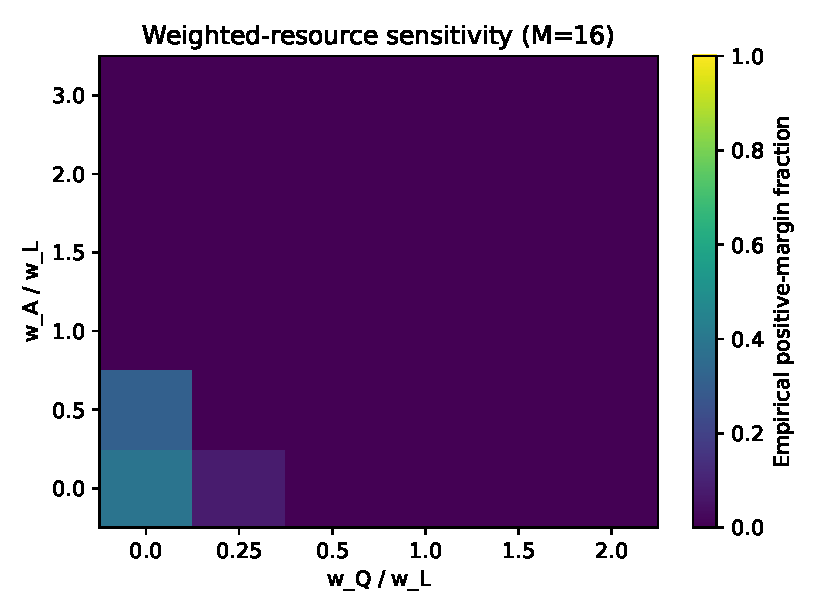
\includegraphics[width=0.86\linewidth,height=0.25\textheight,keepaspectratio]{figures/weighted_resource_sensitivity_heatmap.pdf}
\caption{Weighted scalarized resource sensitivity. The weights are declared comparison conventions rather than hardware calibration.}\label{fig:secondary-weighted_resource_sensitivity_heatmap}
\end{figure}
\begin{figure}[p]\centering
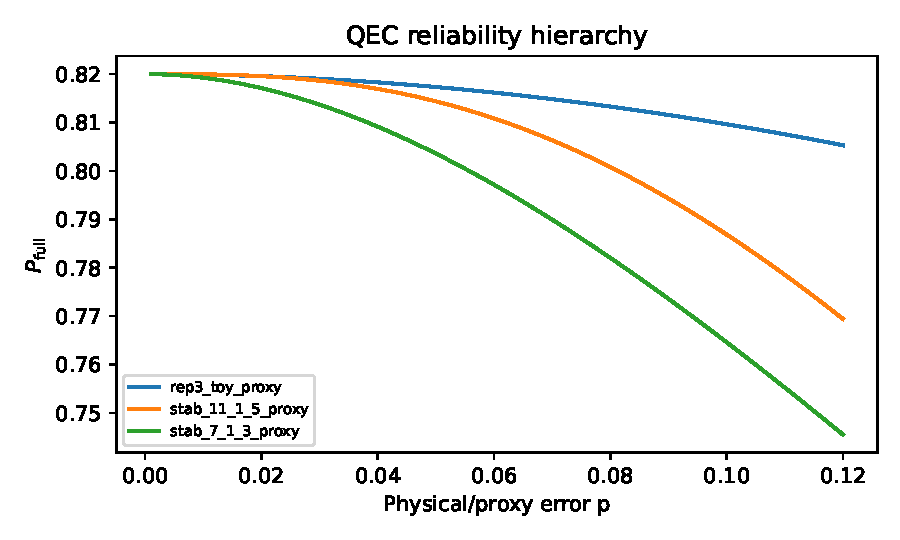
\includegraphics[width=0.86\linewidth,height=0.25\textheight,keepaspectratio]{figures/qec_reliability_hierarchy.pdf}
\caption{Effective logical-failure toy and proxy reliability diagnostics.}\label{fig:secondary-qec_reliability_hierarchy}
\end{figure}
